

\chapter{Introduction to surface forces}

%Intro
%Surface forces - van der waals, electrostatics, charge screening, DLVO, derjaguin
%hydrodynamics - lubriciating, viscous forces
%brownian 
%Rheology - bulk & translation, shear thickening, friction, industry
%MOVE OUR SYSTEM TO CHAPT4
%Conclision

%Check what I define what a long range force is, what is a short range force is?

%add nomenclature/glossary
%Where is Ue(r) defined ?

%REFERENCES ARE BUGGERED PLEASE FIX BEFORE SENDING OFF TO BE READ!!!

 
\title{Introduction}

%The methods of how particles interact with one another has been a longstanding area of interest in physics. As matter encroaches upon one another %there in an interplay of attractive and repulsive forces.
The fundamental interactions between particles has long been an area of active research in physics. The interplay of attractive and repulsive forces which occurs at the boundary between particles is both difficult to understand and vital to master.

%These forces and mechanisms are known as interacting surface forces, and the interplay of these interactions define the systems we experience and observe in day to day life. Some examples include the wetting of surfaces from an interfacing liquid or the means in which an organism adheres to a surface. 
Examples of the emergent behaviour which arises from these interactions includes the spreading of a water droplet across a surface and the adherance of micro-organisms to surfaces.

These forces
%while from the perspective of the universe are nothing new,
have
%gained
recieved increasing interest and understanding over the last century
%to
from scientists and industry alike. The demand for a clear and concise picture of these interactions only increases as innovations in technology rely more and more on these interactions, from touch screen developments, 
%water resistant
superhydrophobic surfaces, bacterial frustrating surfaces or even the humble custard. 

There are several ways to 
%flirt with
probe these forces 
%either as an innovator; 
either by chemically treating the surface, altering the physical structure of said surface or by altering the
%inter-facial 
nature of the 
%solute 
solution said surface finds itself involved with. By changing these properties, new promising technologies can 
%push
advance our understanding of such 
%a
systems.
%to it's limits. 

As %scientific study
researchers become
%s
more and more involved on 
%elucidating
studying these interactions,
%on the molecular scale
 we find more and more of the world we live in is 
%defined by our understanding 
a result of the emergent behaviour of such systems and as a result, it is imperative to not only question the history of our combined understanding, but to test such systems experimentally.

%The history of surface forces finds itself
Our modern understanding of surface forces is derived from van der Waals 
%forces, 
theory,
%a theory produced by 
the result of a series of papers produced by London, Debye and Keesom \cite{AFMvdW}. %These 
Attractive forces were combined with repulsive double layer forces to %form 
give the main theoretical basis %of 
for particle-particle interactions, %consequently 
subsequently %known 
referred to as DLVO theory (derived from Boris Derjaguin and Lev Landau, Evert Verwey and Theodoor Overbeek) as a result of two groups reaching the same conclusion independently\cite{Verwey}\cite{DERJAGUIN}. This underlying theory describes the %resultant 
surface forces felt between two particles in solution .

%From these simple particle-particle interactions bulk behaviours are derived, 
More complex behaviours arise emerge as a result of these interactions - for example %such as the case for 
colloidal systems. Mixed phase suspensions, called colloids are a combination of a solvent and a solute. Indeed, one only has to look inwards to find a fascinating colloidal system (albeit a very complicated one). \cite{surfThesis} \cite{christian2018a}

Systems defined by inter-molecular forces are prevalent in a wide range of applications, said theory providing the basis for several industries such as water purification, batch processing (food, pharmaceuticals, detergents, paints) and mining.\cite{TABOR19772}

%Born from (history)

\section{Forces between molecules}

%wrong - don't trust interpretation 
Inter-molecular forces are essentially electrostatic in nature, as postulated from quantum theory, initially defined by the Hellman-Feynman theorem. %From the Coulomb force and complex fluctuating forces observed around the surfaces of atoms. 
However, %simple solutions to the Schrödinger are hard to come by, 
solving Schrodinger's equation for poly-atomic systems is very difficult and as such, this unified force is fractured down into smaller %classifications 
components to simplify their definition and %equation
computation. These categories are %known as 
ionic forces, van der Waals forces, hydrophobic forces, hydrogen bonding and solvation forces. 

%Covalent / coloumb interactions, short range and strong
Chemical bonding depends on the interaction of neighboring atomic orbitals, while steric forces arise from quantum mechanical or electrostatic interactions between separated particles. %They are an emergent property of the electronic structure of the atoms, as apposed to a molecular orbitals, where the molecular configuration is in a state of semi-perminance and free from flux changes.

%A main difference between the two is the permanence of charge distribution changes, where in the case of the former is retained as long as the bond is retained.

Coulomb's %forces 
law %are 
describes the force %of the charge effects of two charges applied upon one another with respect to distance. 
which arises from the electrostatic interaction of charged particles:

%loose
%In  approximation the inverse square force is given by: %Not atoms per say
%Why is this the simpliest


\begin{equation}
F \propto \frac{Q_1 Q_2}{kr^2}
\end{equation}

Where upon this can be expanded into:

\begin{equation} %\frac{Q_1 Q_2}{4\pi\varepsilon_0\varepsilon r^2} =
F = -\frac{dw(r)}{dr} =  \frac{z_1z_2e^2}{4\pi\varepsilon_0\varepsilon r^2}
\end{equation}

where w(r) is the free energy of the Coulomb interaction, r is the distance between the two charges Q\textsubscript{1} and Q\textsubscript{2}. $\varepsilon$ is dielectric constant of the medium, and z is the ionic valency of the atom in question, in relation to the elementary charge e. % Due to it's inverse square law nature it is a force highly dependant on distance. 
The inverse square relationship between the free energy of interaction and distance between the point charges makes this force drop off sharply as the distance increases.

%w(r) is Joules, ~ 8x10^-19J, kT is 5x10^-21J. Stronk.

%lennard jones potential here?

\section{Brownian Motion}

%Traditionally; 
The term colloid was coined in 1861, drawn from the Greek word $κόλλα$ (kolla), meaning glue, from Thomas Graham's observations of particle aggregation\cite{old_colloid}. %Nowadays 
today, a colloid is defined as %the intermixing 
a mixture of two separate phases; a dispersed, suspended phase and a continuous%, medium
phases in which the former find themselves in. %For our area of interest, we place our scope on a particular colloidal suspension; a dispersion of solid particles within a liquid medium. 
Colloids consisting of solid particles suspended in a liquid medium shall be the focus of this thesis.\cite{review_colloid1}

Consider the idea of marbles kept within a liquid. At rest, they would lie upon the bottom of the container, yielding to the force of gravity\cite{Neuton}. However, as you scale down these marbles, to smaller and smaller sizes, the kinetic energy of the system is enough for keep the marbles dispersed within the liquid, due to Brownian motion\cite{Brown}.

At micrometer sizes however, the marbles begin to affect one another; when two marbles are brought together by Brownian motion, provided the interactions between the two of them are attractive, they will attract towards each other, and eventually aggregate, until they are large enough to sediment again. If there is no attraction, or indeed repulsion, between the marbles, they will stay suspended within the solution.

%Interactions between the marble's surfaces, are defined by a few fundamental forces resolving linearly with one another. These interplay of forces, borne from electrostatics, van der Waals and solvation forces, all sum up into a force profile based on distance between the two surfaces.

The various interactions between the marble surfaces can be combined to give a force profile, describing the strength of the interaction between the marbles with respect to the distance between them.

These force profiles depend upon a number of % intrinsic 
properties intrinsic to the phenomena. %To define these variables in a broad stroke; the liquid the solid colloid is immersed in (liquid phase properties), the surface properties of the solid phase (solid phase properties) and interactions between same phase particles (same phase interacting properties).


On the macro scale, these interactions %equal out to resolve into their 
ultimatley contribute to bulk properties. As this system is disturbed by external forces, a 
%resultant 
characteristic relaxation time is observed, dependant on the ions in solution and surface properties of the solid phase particles. %From these disturbances, new dipole moments can arise additionally. 
These properties give rise to the %hysteric effects 
time dependent effects seen in systems such as these.

With such a complex system of non trivial interactions, the history of elucidating such a complex system has not been a simple one. Ideally in physics finding a unifying, complete equation to describe all manner of interactions would be the goal, however, even if that were possible, colloidal systems are not frozen in an equilibrated state and are the result of combining relations between intrinsic properties and dynamic, sympathetic effects. As such the current state of the theory relies upon simplified simulations to push forward the field, and as such, an experimental analysis %upon 
 of said models is required. \cite{FoundColloidBook}\cite{IsGreenBook}



\section{Van der Waals Forces}
The %predominant 
strongest attractive forces %applied 
acting %upon 
on the solid phase of a colloidal system %is 
 are described byvan der Waals %attractive forces. 
 theory.

Originally recognised by Johannes Diderik Van der Waals, of which the name derives from, in 1873 \cite{vanderWaals} it was only later in 1930 that these forces were defined by London in 1930\cite{London} almost 60 years later into what is known as London dispersion forces. 

%Honking
These forces can be further broken down into three types;  Keesom forces (aka perminant dipole -perminant dipole interactions), debye forces (aka perminant dipole - induced dipole interactions) and dispersion forces (aka induced dipole - induced dipole interactions). \cite{sciDirBook}. Keesom forces derive from the permanent charge nature of atoms, where a static dipole induces an attraction between two particles, due to their stable differences in charge (see fig \ref{fig:keesom}). These fluctuating motions present in these permanent dipole moments result in the $1/r^6$ interaction potential even with these other sources.

Dispersion forces act between all atoms and molecules, even present in neutrally charged elements, 
%thanks the their 
as a result of the Heisenberg uncertainty principle.\cite{}
%quantum mechanical nature. 
To explain how these forces arise, consider an atom. While the time averaged dipole moment is zero, due to %the changing position  of its electrons around it's positively charged nucleus, 
fluctuations in the electron density around the nucleus, a %it has a fluctuating n
on-zero, instantaneous dipole moment is present. This fluctuating instantaneous dipole moment generates a fluctuating electric field on any neighboring neutral atoms. The interaction between the instantaneous dipole moment in %atom one and the induced dipole in atom two, 
one atom and the induced dipole in another, averaged over orientation to account for the fluctuating nature of the instantaneous dipole, gives rise to an attractive interaction between the two atoms. The intensity of the induced electric field from instantaneous dipole moments falls off with distance as $E_{\rm ins} \propto 1/r^3$, and the induced dipole moment is proportional to this field, $p_{ind} \propto \alpha E_{\rm ins}$ with $\alpha$ to polarizability of the second atom. The interaction energy is then $U \propto p_{ind}E_{\rm ins} \propto 1/r^6$. 
%Break out equations from text

%Move down
These forces have been variously described as dispersion forces, London forces \cite{London} and dipole-dipole forces, all %attributing to their origin;
referring to a dispersion force caused by an electro%dynamical
nic charge flux inducing dipole moment. These dispersion forces make up one of three types of forces contributed by van der Waals forces and% is
are ubiquitous, unlike the other two sources, which depend on their permanent dipole properties and the nature of the medium. \cite{IsGreenBook}

%MAKE SURE TO FIX THE DIAGRAM PRESENTATION/LOCATION THINGIE

\cite{lilBlueBook} \cite{IsGreenBook}  \cite{FoundColloidBook}

%\newpage


\begin{figure}[h!!!!!!!!!!!!!!!!!!!!!!!!!]     %Insert a figure as soon as possible
        \begin{center}
          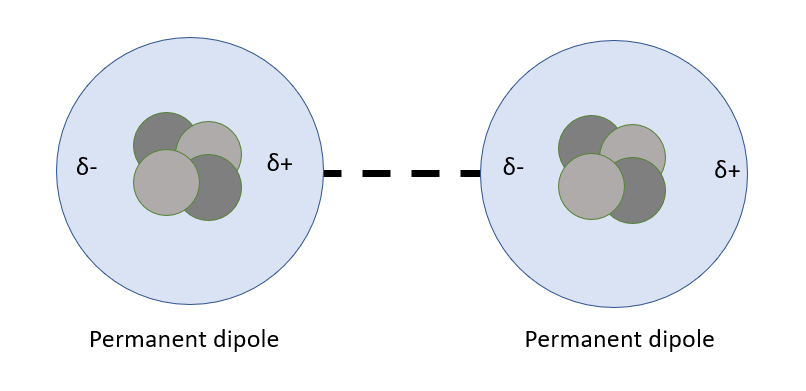
\includegraphics[width=110mm]{chapter1/keesom.PNG}
\end{center}
\caption{A basic schematic of Keesom interacting forces.}
\label{fig:keesom}                 % Reference label to the figure.
\end{figure}



Debye forces %instead
result from the influence of an instantaneous dipole on a permanent dipole%induce a dipole moment in a nearby atom, causing a %sympathetic
%corresponding response from the permanent dipole 
the interaction between the electronic fields results in a force between the dipoles(see fig \ref{fig:debye}). This quantum mechanical phenomena arises from fluctuations %of the electrons on the surface
in electron density, resulting in an averaged $\delta$ positive force on the induced atom, from the localised departure of electrons away from the inducing atom. 

\begin{figure}[h!]     %Insert a figure as soon as possible
        \begin{center}
          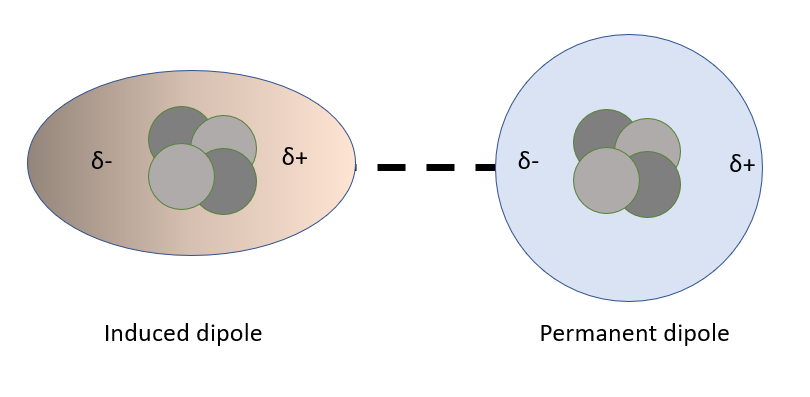
\includegraphics[width=110mm]{chapter1/debye.PNG}
\end{center}
\caption{A basic schematic of Debye interacting forces.}
\label{fig:debye}                 % Reference label to the figure.
\end{figure}

dispersion interacting forces (see fig \ref{fig:disp})

\begin{figure}[h]     %Insert a figure as soon as possible
        \begin{center}
          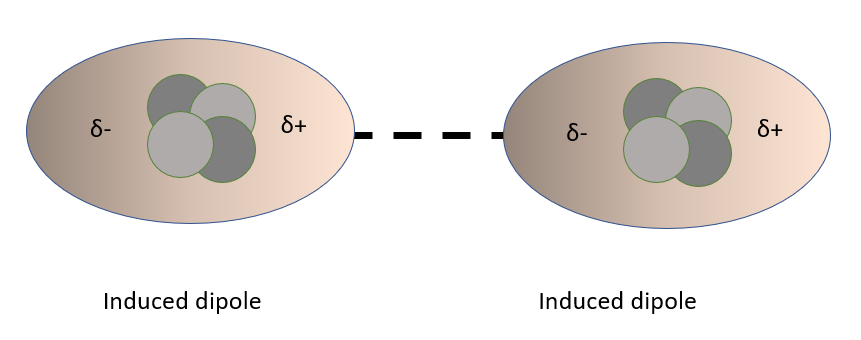
\includegraphics[width=110mm]{chapter1/London.PNG}
\end{center}
\caption{A basic schematic of dispersion interacting forces.}
\label{fig:disp}                 % Reference label to the figure.
\end{figure}

Van der Waals forces make up the dominant short-range attractive force between macroscopic colloids.\cite{colloid_review1}%, however, the operational distance of the force is very short ranged, as it relies heavily on induced dipole fluctuations on the surfaces between particles.  
This interaction can be described by equation \ref{Hammy}:  

%Fill out - T
\subsubsection{Mathematical basis of dispersion forces} %inseperable

\begin{equation} %Alternative - from excel model paper (Nano focused, misses out on larger particles?) R must be distance then?? (nanocoatings practice and principles)
U_{vdW} (r) = - \frac{A r}{12hkT}
\label{Hammy}
\end{equation}

\begin{equation}
U_{vdW} (r) = - \frac{A}{12\pi} \left( \frac{R}{r}\right)^2
\label{VDWeqn}
\end{equation}

%Maybe consider that Hamaker isn't a constant constant, so to speak
U being the attractive cohesive energy, A is the Hamaker constant, R is the radius of the collodial particle, assumed to be of equal radius for the other particle, r distance between the two particles.\cite{?} A is calculated by:

\begin{equation} %Foundation of collodial science
A = \pi^2 C p_1 p_2
\end{equation}

Where C is the interaction parameter, given by the coefficient in the particle-particle pair interaction. $p1$ and $p2$ are the number densities of two interacting kinds of particles.\cite{?} C is calculated by:

\begin{equation}
w(r) = - \frac{C}{r^6}
\end{equation}

where $w(r)$ is the pair interaction energy between two particles.

One striking element of the %derived 
interactions %energies between colloidal particles is %it's heavy reliance on distance, 
is their short range - significant only %where they are only effective 
up to tens of nanometers. When colloids in a solvent are considered, it is important to note that %A will change with respect to the solvent it finds itself in, and the colloidal particle's properties.
takes on a characteristic value for each colloidal system.\cite{?} %Great where did my citation go


\subsection{Electrostatic interactions} %The repulsive part, unfortunately not in that way.

When two phases %interface with one another 
mix, there is a %known 
tendency for ions to arrange along the %interface
phase boundary, %in order to reduce the free energy of the system. 
as this tends to be the lowest energy configuration. %These resultant electric fields from the ions may induce polarisation effects in nearby molecules. These combined effects result in an electric potential difference between the two phases.
The concentration of ions at the phase boundary produces an electric field, capable of polarizing nearby molecules.

Coulomb's law attempts to explain the force experienced between two electrically charged particles suspended in motion. This force is usually referred to as electrostatic force or Colombic force.

\begin{equation} %Basic principles of colloid science - 39
F = \frac{q_1q_2}{4 \pi e_0 r^2}
\end{equation}

%Fix reference
This law describes the force applied to two particles with electric charge $q$ ($q_1$ and $q_2$ respectively), where $e_0$ is the vacuum permittivity. In the case where the particles are in solution, this is replaced by $\epsilon$ - the dielectric constant, given by: 

\begin{equation} %Basic principles of colloid science - 39
\epsilon =  \frac{e}{e_0}
\end{equation}

%Highlight full equation instead, because prior is for a vacuum, and I've done nothing in a vacuum (Because vacuums are filled with nothing)
Where $e$ is the electron charge. If the sign of $q_1$ and $q_2$ are the same, then it is a repulsive force, otherwise it is attractive. $4\pi \epsilon_0$ is sometimes simplified to the electrostatic constant. 

Charges on surfaces can arise due to several different phenomena:, The innate surface chemistry, the adsorption of ions from the solution onto the surface and dissociation of surface ions into solution.

Surfaces can also be affected by charge in a range of different ways.  Surface chemistry ionisation can occur based upon the solvent pH, where acidic or basic groups% can dissociate away from the surface and into the solution. 
are ionised according to the pH of the solution . %The surface has a positive charge in the case of a basic surface, and a negative in an acidic. One way to manage this property is to control the pH of the solution. %other 4 factors don't really impact the setup, except maybe ionic absorption at a stretch

The charge present upon a surface attracts counter ions, which associate towards said surface. This phenomenon is known as charge screening and is dependant on ionic salts within the aqueous solution.
\cite{babthes}%33 34 52

\subsubsection{Charge screening}

%add eqns and pictures pls

As %ions
ionic species diffuse %seek to stabilise themselves 
within a solution %and 
tending towards a %reduce 
reduction in the free energy of the system, %an ionic atmosphere surrounding any inversely charged surface will develop over time.
charged surfaces will tend to become surrounded by a cloud of counter-ions of opposing charge. %Counter ions will move towards the attractive force from the surface, while same charge-ions will be repelled away from the surface. 
This resulting atmosphere is often referred to as the electrical double layer. %As these ions rely on thermal motion to graduate towards the negative surface, it is this thermal energy that causes the ions on the surface to diffuse slightly from direct contact.

One way to reduce the charge barrier from the surface is to introduce an contrary charged ion, inverse of the colloidal surface charge, to the liquid medium. As these ions stabilise in the system they are inevitably attracted towards the counter charged surface of the colloid, and settle around them as a "cloud". Thus, the concentration, charge and valence of the ionic salts will change the repulsive forces upon interacting colloids.\cite{?} 

\begin{figure}[h]    
        \begin{center}
          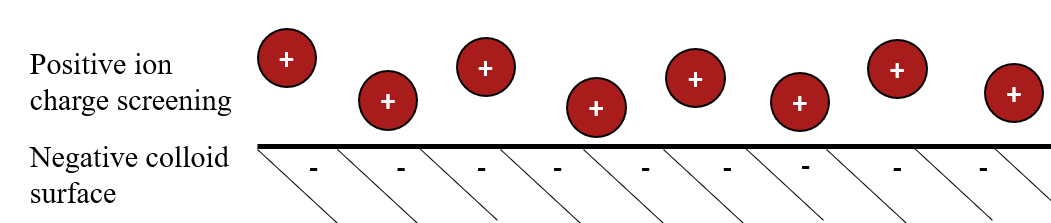
\includegraphics[width=110mm]{chapter1/ioncloud.PNG}
\end{center}
\caption{A schematic of counter ion distribution under the Gouy-Chapman model. This demonstrates how positive counter ions will arrange themselves around a negative surface.}
\label{fig:ioncloud}                
\end{figure}

%Foundations of colloid science
These ions are subjected to an electrostatic potential ($\Psi$) as they get closer towards the oppositely charged surface. The positive counterions (see fig \ref{fig:ioncloud}) are attracted by the electric field generated from the negatively charged surface producing a potential seen in fig \ref{psi}. 

\begin{figure}[h]    
        \begin{center}
          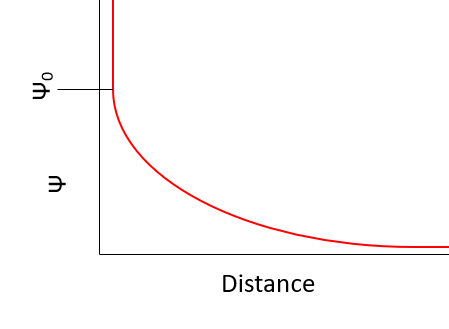
\includegraphics[width=80mm]{chapter1/psi.PNG}
\end{center}
\caption{The Electrostatic potential of a counter ion, where distance is the distance between the negative surface and positive ion.}
\label{fig:psi}                
\end{figure}

%Volta and Galvani potentials (inner and outer) - though maybe not exactly needed. Mostly interested in the double layers interacting.

In addition to this attractive force upon the ion, the ions are additionally subjected to thermal motion. This thermal motion distributes said ions uniformly throughout the aqueous solution. The result of these combined forces is that the surface of the colloid is surrounded, but not saturated, by said counterions, where they gradually reduce in concentration until reaching bulk concentration levels. This phenomena is termed the diffuse electrical double layer which is highly dependant on the electrolytes in solution.

This double layer phenomena has several models attributed to it. One of the earliest theories put forwards was the Helmholtz model in 1853. This theory puts forward the idea of a simple charge distribution contrary to the surface charge along a planar distribution. This distribution is a function of the distance away from the surface, and thus surface charge. While this model provided a basis of understanding the interactions between solvent ions and surface charges as a function of distance, it was unable to account for the effects of kinetics on the system. Under this system it was anticipated that the counter ion concentration would increase with proximity to the surface charge, with same charge ions inversely affected.

This model was then revised under the Gouy-Chapman model in 1910-1913, \cite{34} which pays respect to the thermodynamic nature of the system. Which relies on a linearised and approximated Poisson-Boltzmann equation %NOT REGARDING LAST EQN (reposition)
which assumes a uniform surface charge. Equally it assumes that the dielectric constant of a solution is homogeneous, implying that all ions form a diffuse point charge layer and thus ignore discrete ion binding sites. 

%Move down later
It is worth noting that the only variables within the equation are from temperature and electrolyte concentration, outside of the constants.

The measure of the effect of this layer The Debye length ($\lambda_D$ or $\kappa^2$) represents the distance beyond which the electrostatic force between charged particles is insignificant.

\begin{equation}
\lambda_D = \kappa^{-1} = \sqrt{ \frac{ \epsilon_r \epsilon_0 k_B T}{2Z^2 e^2 n_b}}
\end{equation}

Where $\epsilon_0$ is the vacuum permitivity, $k_B$ is boltzmann constant, T is  Temp in K) 
$\epsilon_r$ is the relative dielectric constant, e is the elementary charge, Z is the charge number of the ions in solution and $n_b$ is the number density of the ions. %(units $\frac{1}{m^3}$)
The number density is given by:
%(LiCl, NaCl etc at 1:1 electrolytes, so Z=1, if you have multiple types of ions in solution you have to sum up the different contributions, but we don’t need to worry about this)
\begin{equation}
n_b = N_A \frac{moles} {Volume}
\end{equation}

Where $N_A$ is Avogadro's constant. This can be further simplified to:

\begin{equation}
 \lambda_D = \kappa^{-1} = \sqrt{ \frac{ \epsilon_r \epsilon_0 k_B T}{2000N_A e^2 I}}
\end{equation}

Where I (the ionic strength) is calculated using:

\begin{equation} 
I = \frac{1}{2} \Sigma c_i z_i^2
\end{equation}

This characteristic length-scale is then split up into two smaller layers, known as the Stern and diffuse layer.

 %what? Helmholtz was before, not after.
%1853 Helmholtz -> Gouy-Chapman 1910 -> Stern 1924 -> Grahame 1947 -> BDM 1963 -> Trasatti/Buzzanca 1971 -> Conway 1975/80ish -> Marcus 1992 (looks quantum? Electron jump probabilities)
%Rough timeline - not all individual theories
%Overbeek (1952) ->

\begin{figure}[h]     %Insert a figure as soon as possible
        \begin{center}
          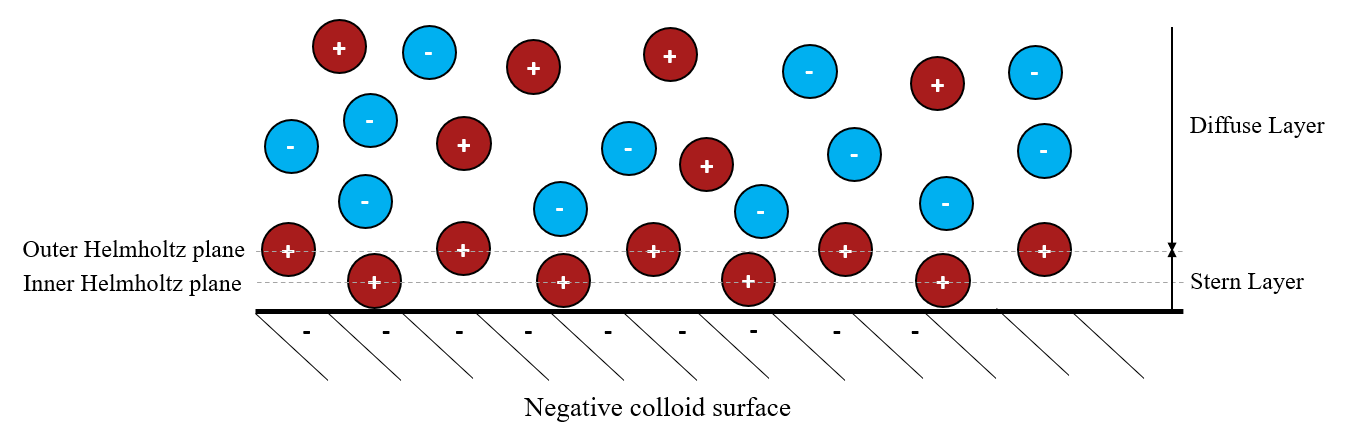
\includegraphics[width=110mm]{chapter1/SternLayer.PNG}
\end{center}
\caption{The Electrical double layer model highlighting the transition between the Stern and diffuse layers.}
\label{fig:Stern}                 % Reference label to the figure.
\end{figure}

The Stern layer is comprised of counterions 

Within this region there is a volume of liquid that is unique to the bulk properties of the liquid phase. This region with a higher concentration of counter ions is called the Helmholtz region and is further split up into two parts. The closest to the surface being the inner Helmholtz plane - where ions are adsorbed onto the surface, and the outer Helmholtz layer contains solvated ions. Afterwards the diffuse layer is made up of unbound free ions influenced by Brownian motion.
%and electrostatics, but that's not unique? 

\subsubsection{Electrostatic repulsion}

%Expand upon double layer interactions

Without the presence of electrostatic repulsion, these particles would surely aggregate together. These repulsive forces arise from the electric charges on the surface of the particle in question, with the strength of these forces varying to the medium they find themselves in.\cite{?} The electrostatic energy of this repulsion is given by:

\begin{equation} %This can't be right??
U_E (r) = 4\pi\epsilon R \Psi^2_{0} \epsilon_0 e^{-\kappa h}
\end{equation}

%h Is separation (old r)
%\color[red]{D is the electric displacement field}
$\epsilon$ being the dielectric constant of the solvent, $\Psi_0$ being the surface electric potential of the colloid, $\sigma$ is the surface charge density and $\kappa$ is the Debye-H\"uckel constant, or Debye length, defined by:

\begin{equation} %General use eqn I see everywhere else Probably just use this, I just need an approx. (2x10^3 bottom term)
\kappa^{-1} = \left(\frac{\epsilon_r \epsilon_0 k_B T}{2 N_A e^2 I}\right)^\frac{1}{2}
\label{eqn:debye} %If you delete this, DO NOT FORGET TO MOVE THIS
\end{equation} %Moles per m^3

\begin{equation}
n_b = N_A (moles /m^3)
\end{equation}

\begin{equation}
\lambda_D = \kappa^{-1} = \sqrt{ \frac{ \epsilon_r \epsilon_0 k_B T}{2000N_A e^2 I}}
\end{equation} %Moles per L

\begin{equation}
\kappa^{-1} = \sqrt{ \frac{ k_b T \epsilon_r \epsilon_0}{2 N_A e^2 I}}
\end{equation}

$e$ being the electron charge, $n_(oi)$ is the concentration and $k_bT$ being the thermal energy of the system (Boltzmann's constant plus temperature) \cite{boltzmann}. The Debye length is the lengthscale of screened electrostatic repulsions.\cite{?}



\begin{equation} %~1 - 100 (50-100 silica ph9) (find ref)
\Psi_0 \approx \frac{\epsilon_r \epsilon_0 \kappa}{\sigma}
\end{equation}
%Find approx sigma value


$c_i$ is the ionic concentration $z_i$ is the valence of $_i$ ions.

\subsection{Lennard-Jones potential} %Mostly bulk? Not sure if needed.
%Give a history lesson not a maths lesson

%Pauli - electron spin repulsion (possible to have two electrons on the same quantum state due to electron shell overlap - this leads to repulsion)
One of the simpler ways to model particle-particle interactions is using a Lennard-Jones potential. This originally seeked to model interactions between two noble gas atoms by describing Pauli repulsion coupled with an attractive long range term. This provides a simplistic view by assuming all interactions between all particles are the same, and thus the solution is homogenous. This is done by summing the contributions from all particles interacting with one another. For each interaction the attraction is given by the Van der Waals attraction (See equation \ref{VDWeqn}). The repulsive term is given by:


Further simplification can be done in the following form \cite{lilBlueBook}:
%rewrite: Which can be simplified to:

\begin{equation} %Basic principles of colloid science
U = 4 \epsilon_{min} \left[\left(\frac{r_0}{r}\right)^{12} - \left(\frac{r_0}{r}\right)^6\right]
\end{equation}



This removes the need for the $A$ and $B$ constants, instead expressing the relationship using the depth of the potential well ($\epsilon_{min}$) and the distance at which the potential is 0 ($r_0$).  

\begin{figure}[h]     %Insert a figure as soon as possible
        \begin{center}
          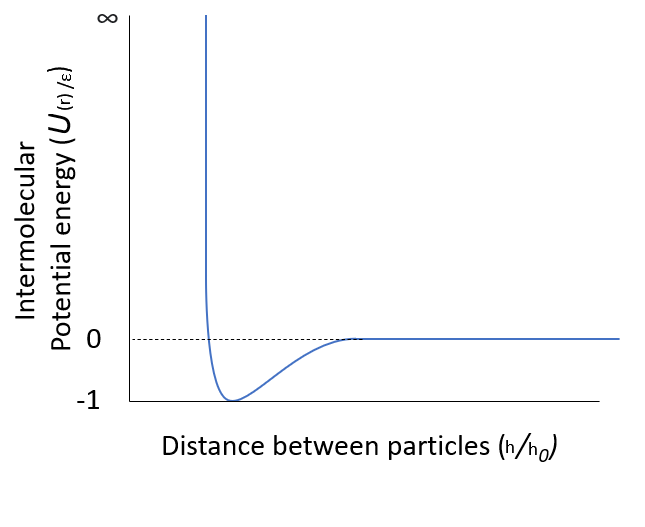
\includegraphics[width=110mm]{chapter1/Lennard's potato.PNG}
\end{center}
\caption{The Lennard-Jones potential function. The potential energy between the two particles is given as a function of distance. As the particles begin to get closer, the experience attraction. As the distance between the two shortens, the attraction eventually gives way to a infinitely increasing repulsive force.}
\label{fig:potato}                 % Reference label to the figure.
\end{figure}

While Lennard-Jones potentials give a good estimation of bulk effects of molecules interacting, it has several limitations. For one it requires homogeneity of both molecules, as well as ignoring any solvent effects. Additionally, it's estimation is independent of charge, which plays a larger role when ions within the solvent are present. In particular the Hamaker constant and $A'$ is derived assuming vacuous conditions, whereas it is known that particles immersed within a solvent experience a reduced attractive force. \cite{} %Find a paper to support this, just in case. What do you mean you don't have one past me??

%In order to improve upon the basics laid out here, these factors need to be considered mathematically. To this end, electrostatics are introduced and considered.

\section{DLVO theory}

These electrostatic $U_E(r)$ repulsions interplay with the van der Waals attractive forces, producing a sum force upon the colloid. This interaction, much like a dance, sways back and forth between attractive and repulsive dominant forces. These two forces were unified into a single theory known as Derjaguin, Landau, Verwey and Overbeek theory (DLVO), named as such based upon the authors in 1943 and 1948.\cite{DLVOorign} \cite{Origin2V} \cite{DERJAGUINORIGIN}

The context of the initial theory was done upon lyophobic colloids, which is to say a collodial suspension of particles in a medium that does not precipitate. Particles are prevented from merging (coalescence) and separating via repulsive forces present between one another, and as a result in an equilibrated state it is stable. This repulsion is produced due to the repulsive electrostatic forces described in 1.1.2, present due to the surface charges of the colloid. The attractive forces of the equation result from van der Waals forces present from the electron distribution of the atomic core, from the molecular surface of the colloid, described in 1.1.2.\cite{DLVOthesis}

These two forces combine to produce a defining interaction potential.

%I'm not green with it
\begin{figure}[h]     %REDO THIS CURVE IT IS BAD AND YOU'RE NOT COMFORTABLE WITH IT
        \begin{center}
          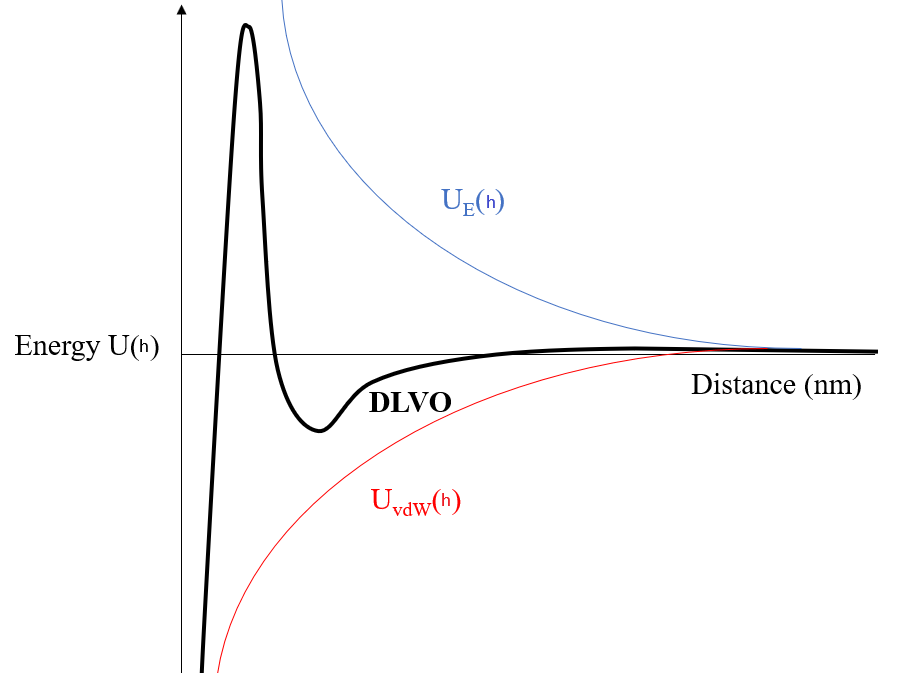
\includegraphics[width=110mm]{chapter1/DLVO.PNG}
\end{center}
\caption{A graphical demonstration of the competing forces between collodial particles. The electrostatic repulsion ($U_E(r)$) and the van der Waals attraction $U_{vdW}(r)$ combine together the sum interplay known as DLVO theory (bold line).}
\label{fig:DLVO}                 % Reference label to the figure.
\end{figure}

One common feature of DLVO is the repulsive barrier that is seen from the initial dip. This energy barrier prevents colloids from agglomerating. The van der waals forces are generally attractive due to the nature of their interactions at longer ranges, giving rise to the inital dip, before the electrostatic repulsion dominates, giving said barrier. However, after this energy barrier is broken, the attraction descends to infinity, demonstrating a very strong attraction. If this barrier is enough to prevent colloids from naturally overcoming it due to Brownian motion and thermal energy, then they will remain stable in solution, though, given infinite time it is likely that the solution will aggregate and settle in it's lowest energy state where $r = 0$, assuming a perfect sphere.\cite{?}

While DLVO has proven itself a functional and applicable model for the description of interacting colloids, there remains a few assumptions that can cause a divergence from the truth. DLVO assumes that the interacting surfaces is perfectly flat, expanding in all directions, and that the surface charge density is uniformly distributed along said surface. Additionally, it assumes that the surface electric potential is constant, and that any counter ions remain static and uniformly distributed too, with any interactions between said ions or solvent being purely born from their dielectric constant. While some of these assumptions aren't true for particle-particle interactions, DLVO holds up as a theory for predicting interactions. \cite{particledep} \cite{effectHetSurf} \cite{colloidDepKin} \cite{chemDiscCharge} \cite{DLVOreview} 

However since this assumes that the interacting objects are flat planes, and not spherical objects. In order to apply this theory to spherical objects their geometry has to be considered. To this effect the Derjaguin approximation is used to approximate the DLVO force between differing geometries.

\subsubsection{Derjaguin approximation}

%THIS IS DEYAGUIN APPROX PLS
The force $F$ experienced by two interacting colloidal particles is given by the free energy ($W$) of two plates  per unit area with respect to the distance between the two ($h$). 

\begin{equation} %colloid.ch
F(h) = 2 \pi r_{eff} W(h)
\end{equation}

Where $R_{eff}$ is the effective radius given by:

\begin{equation} %colloid.ch
r_{eff} = \frac{r_1r_2}{r_1 + r_2}
\end{equation}

Where $r_1$ and $r_2$ are the radii of the two particles. In systems where the radius is homogeneous $r_{eff}$ can be modified to $\frac{r}{2}$. For a system with a sphere and a plane, $r_{eff}$ can be altered to simply equal $r$.

\begin{figure}[h]     %REDO THIS CURVE IT IS BAD AND YOU'RE NOT COMFORTABLE WITH IT
        \begin{center}
          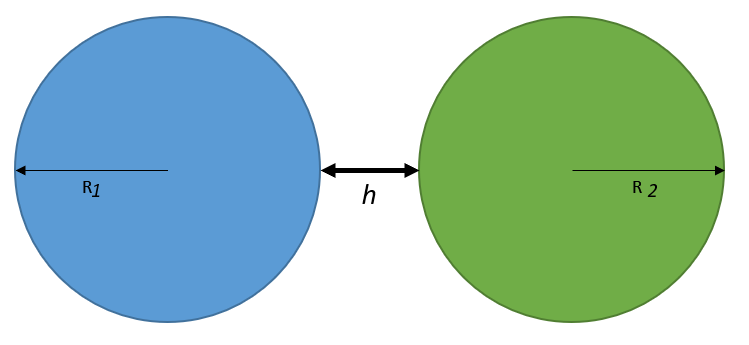
\includegraphics[width=110mm]{chapter1/h_graph.PNG}
\end{center}
\caption{A graphical representation of $h$.}
\label{fig:h_graph}                 % Reference label to the figure.
\end{figure}

This approximation holds up when the size of the interacting particles is relatively larger compared to other force magnitudes present in the system. 

\cite{DLVOsmolOverview, smolBook1}

%\subsubsection{Calculating the Interacting forces}

\cite{DLVOsmolOverview, smolBook1, Origin2V, IsGreenBook}

%please
\cite{surfpattQ} \cite{Surfquestion} 

%




%%See other file - what other file?? Was I drunk writing this??

\section{Hydrodynamic interactions}
The forces discussed prior outline forces that occur when no external forces are applied to the system, and as such the thermodynamical properties are kept time dependant. However, if a force is applied upon the system, then it induces movement locally, and this force precipitates into the rest of the system via hydrodynamical effects. (fig) As the particles within a fluid move, they leave a flow in their wake, which exhibit a force upon other particles and the containing object.

Assuming there is a force applied within the system, this can precipitate out into the rest of the system and can be calculated, provided that one of three assumptions can be made linear flow and constant velocity \(V_o\). 

The force applied upon any single particle under those conditions is given by:

\begin{equation}
F_H = 6 \pi \eta \alpha v_0
\end{equation}

$\eta$ being the intrinsic viscosity of the fluid. $F_H$ is also known as the Stokes drag, provided that the colloidal particles have enough distance to ignore any interparticle hydrodynamic effects.\cite{?}

\subsubsection{Steric forces}

%Other potential sources of long range forces that can have an effect on particle-particle interactions can be drawn from steric forces.

The other way to alter colloid-colloid interactions is to sterically hinder them. By frustrating attractive movement towards one another, they are physically unable to come into contact, and therefore descend towards $r = 0$. Generally, steric hindrance arises from polymeric brushes chemically grafted upon the surface of the colloid, but can also arise from larger molecules in the medium interacting with the surface. For polymeric attachments, they reach our of the colloid as an attempt to reduce the free energy in a system, giving rise to the colloquialism known as polymer brushes. This loss in entropy caused by the brushes frustrating the colloid's freedom of movement causes an increase in the free energy of the system, inciting the colloid's movement away from the other interacting one. Additionally, molecules and particles upon the surface can physically prevent movement of particles towards each other, preventing $r$ from reaching 0.\cite{?}

\begin{figure}[h]     %Insert a figure as soon as possible
        \begin{center}
          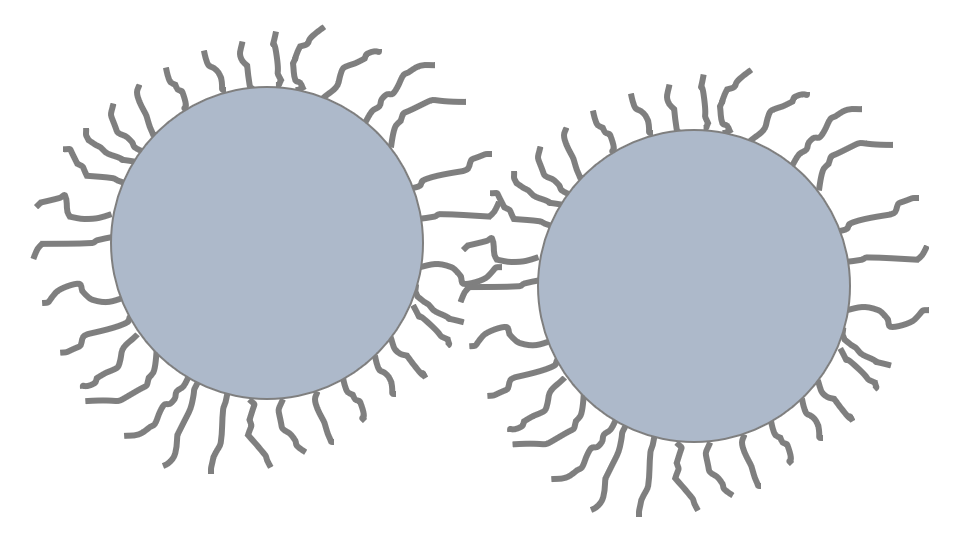
\includegraphics[width=110mm]{chapter1/brushy.PNG}
\end{center}
\caption{The polymers off the surface of the colloid sterically inhibit any interactions.}
\label{fig:brushy}                 % Reference label to the figure.
\end{figure}

These intermolecular forces define how particles interact on the micro scale, summing into a distance-force profile between particles. As you draw the scope out from two particle interactions, towards macroscale, multibody systems, you start to enter the realm of rheology.

%sedimentation of salt?

\section{Considering reality}

Whenever considering a mathematical model of reality it is always worth testing it against an assumed case to see whether or not it would hold up. One such case would be to calculate the maximum size of a spherical particle that could hold itself up to a roof under its own attractive force.

\subsection{Attaching a marble to the ceiling}

In this instance, lets consider a marble held up to the surface of the ceiling and calculate the maximum size that it would stay there under it own attractive van der Waals forces. Starting from the simple equation of $F = ma$ we simplify our equation down to a rough order of magnitude calculation.

\begin{equation*}
    \begin{split}
    mg &= F_{vdW} \\
    \rho \frac{4}{3} \pi a^3 g &= \frac{A_H a}{6 h_{m}^2} \\
    \rightarrow a &\simeq \sqrt{\frac{3 A_H}{24 \pi \rho g h_{m}^2}} \\ 
    &\simeq \sqrt{\frac{10^{-20}J}{24 (200kg/m^3) (10m/s^2) (10^{-10} m)^2 }} \\
    &\simeq 1.4mm
    \end{split}
\end{equation*}
\newpage

Where $m$ is the mass of the particle, $g$ is the force due to gravity, $A_H$ is the area of the sphere, $h$ is distance between the surfaces, $p$ is density and $a$ is the area of contact.

%Why did I make this
\begin{figure}[h]     %Insert a figure as soon as possible
        \begin{center}
          \includegraphics[width=110mm]{chapter1/Sphere_on_roof.png}
\end{center}
\caption{A diagram demonstrating a 1.4mm diameter sphere attached to the ceiling.}
\label{fig:disp}                 % Reference label to the figure.
\end{figure}

Given that the area of contact would be 1.4mm, the actual size of the sphere would be much larger, which w


\subsection{Attaching spherical putty to the ceiling}

However, one other consideration can be made about the system described. If a sphere of putty is brought to a ceiling, we know that is capable of adhering to the surface in defiance of gravity. This simple observation lends itself to the consideration that the underlying model is missing a component of reality.

Due to the fact that putty is a pressure-sensitive adhesive, and is viscoelastic, it's area of contact is pliable to rough areas. One issue with DLVO theory is that all interacting geometries are assumed to be flat, which is is a simplification from reality. As all surfaces in reality are %topologically devious 
subject to significant topological deviations, DLVO is not always a perfect explanation of the underlying effects. Indeed, all it takes it one look at it's descent to infinite force at decreasing distances to see an issue. That being said the question then remains, where does the deviation from reality arise from, and can we incorporate it into the model?

Additionally from these single particle interactions comes a wider array of interactions when the scale of the system expands to accommodate multiple spheres interacting with one another. It is from these interactions that the study of Rheology comes into play. 

\newpage

\section{Bulk vs singular interactions}
%review section
\subsection{Rheology}

 As these small scale forces are applied to one another, across the bulk of the solution, with multiple forces applied from multiple directions, the overall clarity of the forces at play begins to obfuscate. It becomes very difficult to observe in detail the individual mechanisms of particle-particle interactions. As such, either rheological techniques are used for in vitro examination, or the in use of simulations. Rheology itself studies the flow and deformation of a bulk liquid solution under different forces, of which colloids are known the play a part. Oobleck, a well known solution, displays shear thickening properties under shear stress, born from the interplay of forces between the collodial nature of the solution.
 
 The types of rheological fluids that are created from collodial particles suspensions are known as non-Newtonian fluids. These distinct themselves from Newtonian fluids by not following Newton's law of viscosity. Instead they derive their behavours from the interactions between the suspended particles and from the effects from the suspending medium. Because of this, they are known to have interesting properties \cite{Rheo2}
 
 \subsection{Shear thinning and thickening}
 
 Shear thickening occurs when disperse colloidal particles are subjected to a high shear force, leading to an increase in the observed viscosity. Shear thinning consequently is when the same suspension decreases it's viscosity from shear forces. While it may be intuitive to expect that the effects draw from the same mechanical interaction, it has yet to be proven. The current theory is that shear thinning derives from small structural changes in the suspended system. 
 
 %TODO: add image from edinburgh
 
 Shear thickening on the other hand has two theories regarding it's behaviour. Hydroclustering, which is when a grouping of particles temporally immobilised by a compression event, where their geometries mesh together, preventing further compression. It is this sudden emergent compositional jam that causes the particles to act as a single in-compressible geometry in the suspension. This new geometry affects the resultant flow and therefore viscosity of the suspension. \cite{hydroshock}
 
 The other is a order to disorder transition which the ordered flow transitions to a state of disorder between the particles. This is due to the force applied to the particles overcoming the repulsive barrier between particles so that they come in contact. This then perturbs the liquids flow from the change in structure resulting in a higher viscosity. \cite{ShockCrash}
 
Both of these theories rely on Also mention that these interactions are determined by intermolecular forces on the nanoscale.
 


\cite{SmartMats, Rheo2}

\subsection{Lubrication forces}

Lubrication forces are thought to be the dominant force regarding intercollodial interactions, causing their observed behaviour and structure (for systems with a high colloidal concentration). These forces arise from small, thin lubricating layers between two particles. This this layer is thought to prevent physical contact, and thus frictional forces, between two interacting colloids. From this postulation, the infinite force at R = 0 problem is solved, as the colloids never come into contact, instead separated by thee viscous, lubricating layer between them during floculation. Because of this, the particles are able to separate when the shear force is removed, giving the characteristic viscosity shift back and forth.

?


However it is important to note that this theory relies on said particles being perfectly spherical.

\subsection{Simple viscous drag}
    


    
\subsection{Rheology of suspended collodial particles}

As you scale up the viscosity of a liquid and start applying these forces from the microscale to a collective sum on the macroscale you start to see interesting behaviours arise from the fundamental forces intrinsic to the 


 
 While Rheology relies on deriving it's understanding of such systems from a macroscopic lense, simulations takes the current theory underpinning current scientific understanding to build up a theoretical landscape imitating reality. This in silico landscape often relies on equations use to simulate particle-particle interactions across all of the simulation. Simulations work by drawing a defined box with either periodic or constrained boundary conditions, in two or three dimensions, where each particle's sum force is calculated base upon the other particles within the box. Then, afterwards, the frame of reference is shifted forwards a certain amount of time, with the particle's positions moved based upon the last frame's force. This tick happens over and over, with the total time and accuracy dependant on the delta timestep.\cite{foss_brady_2000}
 
As a result it is important to experimentally verify the results of simulations as the limits of mathematical models can influence the results. As such it is a power visualising tool to express how a system is expect to function, and thus provides a incredible hypothesis generating tool.

\newpage



